\note{Brief Overview}{
These activities provide more practice applying the Energy-Interaction Model to both �weird� physical phenomena as well as to mechanical, as opposed to strictly thermal, phenomena. The last Activity provides an introduction to the spring-mass oscillator. 
}

\section{Modeling with Mechanical Energy Systems}
\note{Timing: \unit[\about35]{min}}{
Purpose:
\begin{itemize}
	\item Intro to two common mechanical energy systems: gravitational PE and translational KE.  
	\item Practice using the energy-interaction model with mechanical energy systems: making inferences and comparing with observation.
\end{itemize}
This is the students� introduction to gravitational potential energy and translational kinetic energy.  Note that we are not getting quantitative in this \DL{} activity; being quantitative comes in the 2nd Concept Group of this unit.  It is important for students to realize that we use exactly the same energy modeling approach with mechanical energies as we did in Unit 1.  This is a central point that you can emphasize.

General Notes:
\begin{itemize}
	\item Try to get groups to do their work at the board!
	\item Tell students to read the initial and final states carefully!  They often have problems with the notions of �just after� and �just before� notions so spend some time here and in the future on this.

	\item Emphasize going from observation to energy systems.  If students observe a change in the object�s position or motion, the object�s energy has changed.  Most groups will probably use potential and kinetic energy systems, but at this point if they have a �system for moving� and �system for position� (or some other name) that�s fine.  During whole-class discussions you can make the official names clear, but continue to refer occasionally to energies of motion and of position.
\end{itemize}

Learning Outcomes:
\begin{itemize}
	\item Know how to use and be confident in using mechanical energies in the Energy-Interaction Model. .
	\item Know how to decide whether internal energy changes are present in phenomena involving mechanical phenomena and how to incorporate this knowledge in applying the Energy-Interaction Model 
\end{itemize}
}
\label{act2.1.1}

\begin{overview}

\textbf{Overview:} After spending the first few weeks of the semester discussing and making sense of various \emph{thermal} phenomena, we now shift our focus to \emph{mechanical} phenomena. We'll start with some new definitions and then immediately dive into some examples.
	
\end{overview}

\subsection{Internal Energy and Mechanical Energy}

\begin{reading}

\noindent At this point, it is useful to define and distinguish two different \emph{types} of energy systems. Make sure the definitions make sense to everybody in your group!\\

\noindent\textbf{Internal Energy}:  Internal energy systems are closely related to the {\em motions} of and {\em relationships} between {\em individual atoms and molecules}. Thermal Energy and Bond Energy are examples of internal energy systems.\\

\noindent\textbf{Mechanical Energy}: Mechanical energy systems have {\em indicators} involving the {\em position} or the {\em speed} of the {\em object as a whole}.  The object can be anything from an airplane to an atom.\\

\noindent\textbf{Important}: Some physical phenomena (such as the thermal phenomena we've dealt with, so far) involve changes {\em only} in internal energy systems, while some phenomena involve changes \emph{only} in mechanical energy systems. Other phenomena involve changes in \emph{both} mechanical and internal energy systems.
\end{reading}

\WCD 

\subsection{Phenomenon: Dropping a golf ball}
\label{actdropagolfball}
\note{Equipment needed at each table:}{
\begin{itemize}
	\item one coffee filter (10 cup size, flat bottom style)
	\item one 200 gram weight (from box set)
	\item hanging brass spring
	\item one two-meter stick with slider (pointer)
	\item one golf ball
\end{itemize}
}
\note{Specific Notes for \ref{actdropagolfball}}{
\begin{itemize}
\item They can see that the height changes and the speed changes (not moving to moving). Emphasize these are the indicators.  Potential and kinetic energy systems are the only ones that have significant change, because we assume that effects of friction and energy transferring to thermal systems are negligible for the heights and speeds involved with the dropping ball.  (You can ask students if this would be true if you dropped the ball from the roof of some tall building.)  We are introducing the labels internal and mechanical energies here.  Bring this out in the \WC{} discussion.
\item There is just the KE and $PE_{gravity}$ (since there will be lot�s of PE�s, get them used to writing subscripts now).  KE? (clearly, since we go from no speed to some) and so $PE_{gravity}$?.  Equation expressing total conservation of energy: �KE + �$PE_{gravity}$ = 0.  Initial height is greater than the final height.  Initial speed (zero) is slower (lower) than final speed (moving faster).
\end{itemize}
}
Drop a golf ball from about one meter above the floor and observe its motion and position.  Focus on the motion and position between the \textbf{beginning} and \textbf{end} states defined below. If you do not have names of energy systems associated with the changes you observed, you can just make up names for these energy systems for now.

\begin{center}
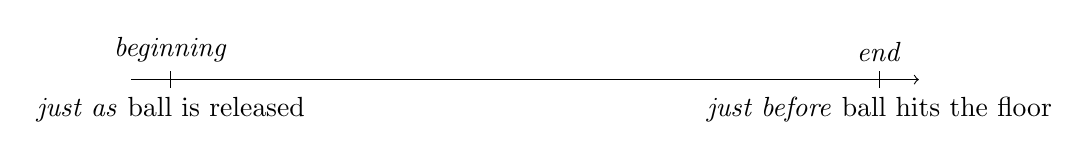
\begin{tikzpicture}
    % draw horizontal line   
    \draw[->] (0,0) -- (10,0);

    % draw vertical lines
    \foreach \x in {0.5,9.5}
      \draw (\x cm,3pt) -- (\x cm,-3pt);

    % draw nodes
    \draw (0.5,0) node[below=3pt] {\emph{just as} ball is released} node[above=3pt] {\emph{beginning}};
    \draw (9.5,0) node[below=3pt] {\emph{just before} ball hits the floor} node[above=3pt] {\emph{end}};
\end{tikzpicture}
\end{center}

\begin{enumerate}
	\item Write on the board: What properties of the physical system (indicators) do you think change \textbf{significantly} between the initial and final state?  What energy systems are associated with those indicators?  Are these \emph{internal} or \emph{mechanical} energy systems, or both?
	\item Put a complete \EnergyDiagram{} on the board.  Show with an arrow if each energy system increases or decreases. Include initial and final values of the indicators.
	\item Write an algebraic representation of your \EnergyDiagram{} that expresses energy conservation in terms of the changes of energy of the relevant energy systems.  
\end{enumerate}

\WCD 

\note{Specific Notes for \ref{actdropcoffeefilter}
}{
\begin{itemize}
\item Since the initial state of the coffee filter is one second after being dropped, it has already reached a constant speed (terminal velocity).  Convincing students that it is not increasing its speed can be a challenge.  Once they see this, they should realize that there is no change in the filter�s KE.  There is a decrease in $PE_{gravity}$ and there is an increase in the Ethermal of air and paper.  These are the only two energy-systems that have significant change.  Now we have both internal and mechanical energy systems changing.
\item There is just the $PE_{gravity}$ and Eth.  $PE_{gravity}$ $\downarrow$ and $E_{th}$ $\uparrow$.  Conservation of energy: $\Delta E_{th} + \Delta PE_{gravity}$ = 0.  Initial speed is the same as the final speed.  Initial $PE$ is greater than final $PE$.  Note: Changes in the thermal system are inferred rather than observed in this case.
\item Air friction is negligible for the golf ball but not for the coffee filter.  This is a function of the frontal area of the object (directly proportional) and the mass of the object (inversely proportional).  You can call on individuals or on small groups to respond.  Emphasize the usefulness of energy-system diagrams for getting at the relevant information needed to think about situations involving things that interact, regardless of the kind of interaction or the energy systems involved.
\item The point is that $PE_{gravity}$ depends on direction, but $KE$ does not.  (We will emphasize this again in the next activity).  Once they�re convinced that direction of movement doesn�t matter, ask if the correct indicator is speed or velocity?  Get them to use speed with energy. 
\end{itemize}
}

\subsection{Phenomenon: Dropping a coffee filter}
\label{actdropcoffeefilter}
Drop a basket type coffee filter from a height of about two meters.  Release it oriented as shown in the figure.

\begin{center}
	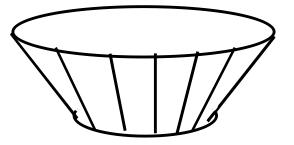
\includegraphics[width=0.25\textwidth]{act211-coffeefilter}
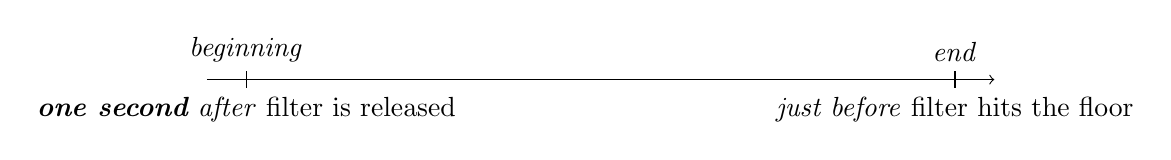
\begin{tikzpicture}
    % draw horizontal line   
    \draw[->] (0,0) -- (10,0);

    % draw vertical lines
    \foreach \x in {0.5,9.5}
      \draw (\x cm,3pt) -- (\x cm,-3pt);

    % draw nodes
    \draw (0.5,0) node[below=3pt] {\emph{\textbf{one second} after} filter is released} node[above=3pt] {\emph{beginning}};
    \draw (9.5,0) node[below=3pt] {\emph{just before} filter hits the floor} node[above=3pt] {\emph{end}};
\end{tikzpicture}
\end{center}

\begin{enumerate}
	\item Repeat part 1 above. Don't forget the last part of the question!
	\item Repeat parts 2 and 3 above.

\WCD 

\subsubsection*{Discuss in your group:}
	
	\item Which of the energy systems you have identified depend on only the \emph{magnitude} of the indicator and which depend on {\em both} the \emph{magnitude} and the \emph{sign} associated with that indicator? 
	\item How are your {\em particular models} for the golf ball and coffee filter different from each other?  Be specific.  What physical properties of the objects are responsible for this difference?
	
\end{enumerate}

\WCD 